Esta investigación está vinculada al proyecto ARTEMIS, una iniciativa del grupo de investigación ArtDiTec, cuyo requisito de entrada es haber sido galardonado con una beca de excelencia en U-tad (Centro Universitario de Tecnología y Arte Digital). ARTEMIS está enfocado en el desarrollo de experiencias digitales interactivas basadas en musicoterapia. Estas experiencias se agrupan en una aplicación diseñada para funcionar como un puente entre el terapeuta y el paciente en terapias psicológicas. El objetivo es ayudar a los pacientes a transitar de emociones con connotaciones negativas hacia emociones con connotaciones positivas.

La investigación se ha centrado en la ansiedad infantil y su tratamiento mediante la musicoterapia. Sin embargo, el proyecto ARTEMIS aspira a ser escalable para diferentes grupos de edad y emociones. Inicialmente, se consideró enfocar la investigación en grupos vulnerables como niños y ancianos. No obstante, se encontró que los niños interactúan más fácilmente con entornos digitales, por lo que se decidió que ese sería el punto de partida para ARTEMIS.

Se ha desarrollado e integrado una experiencia en la aplicación con el objetivo de facilitar la transición de un estado de ansiedad a la calma. A lo largo del documento, se explicará cómo se logra esta transición a través de una ordenación rítmica que pasa del caos al orden subjetivo, mediante la interacción del paciente con las instrucciones proporcionadas por el terapeuta.

\begin{figure} [h!]
	\centering
	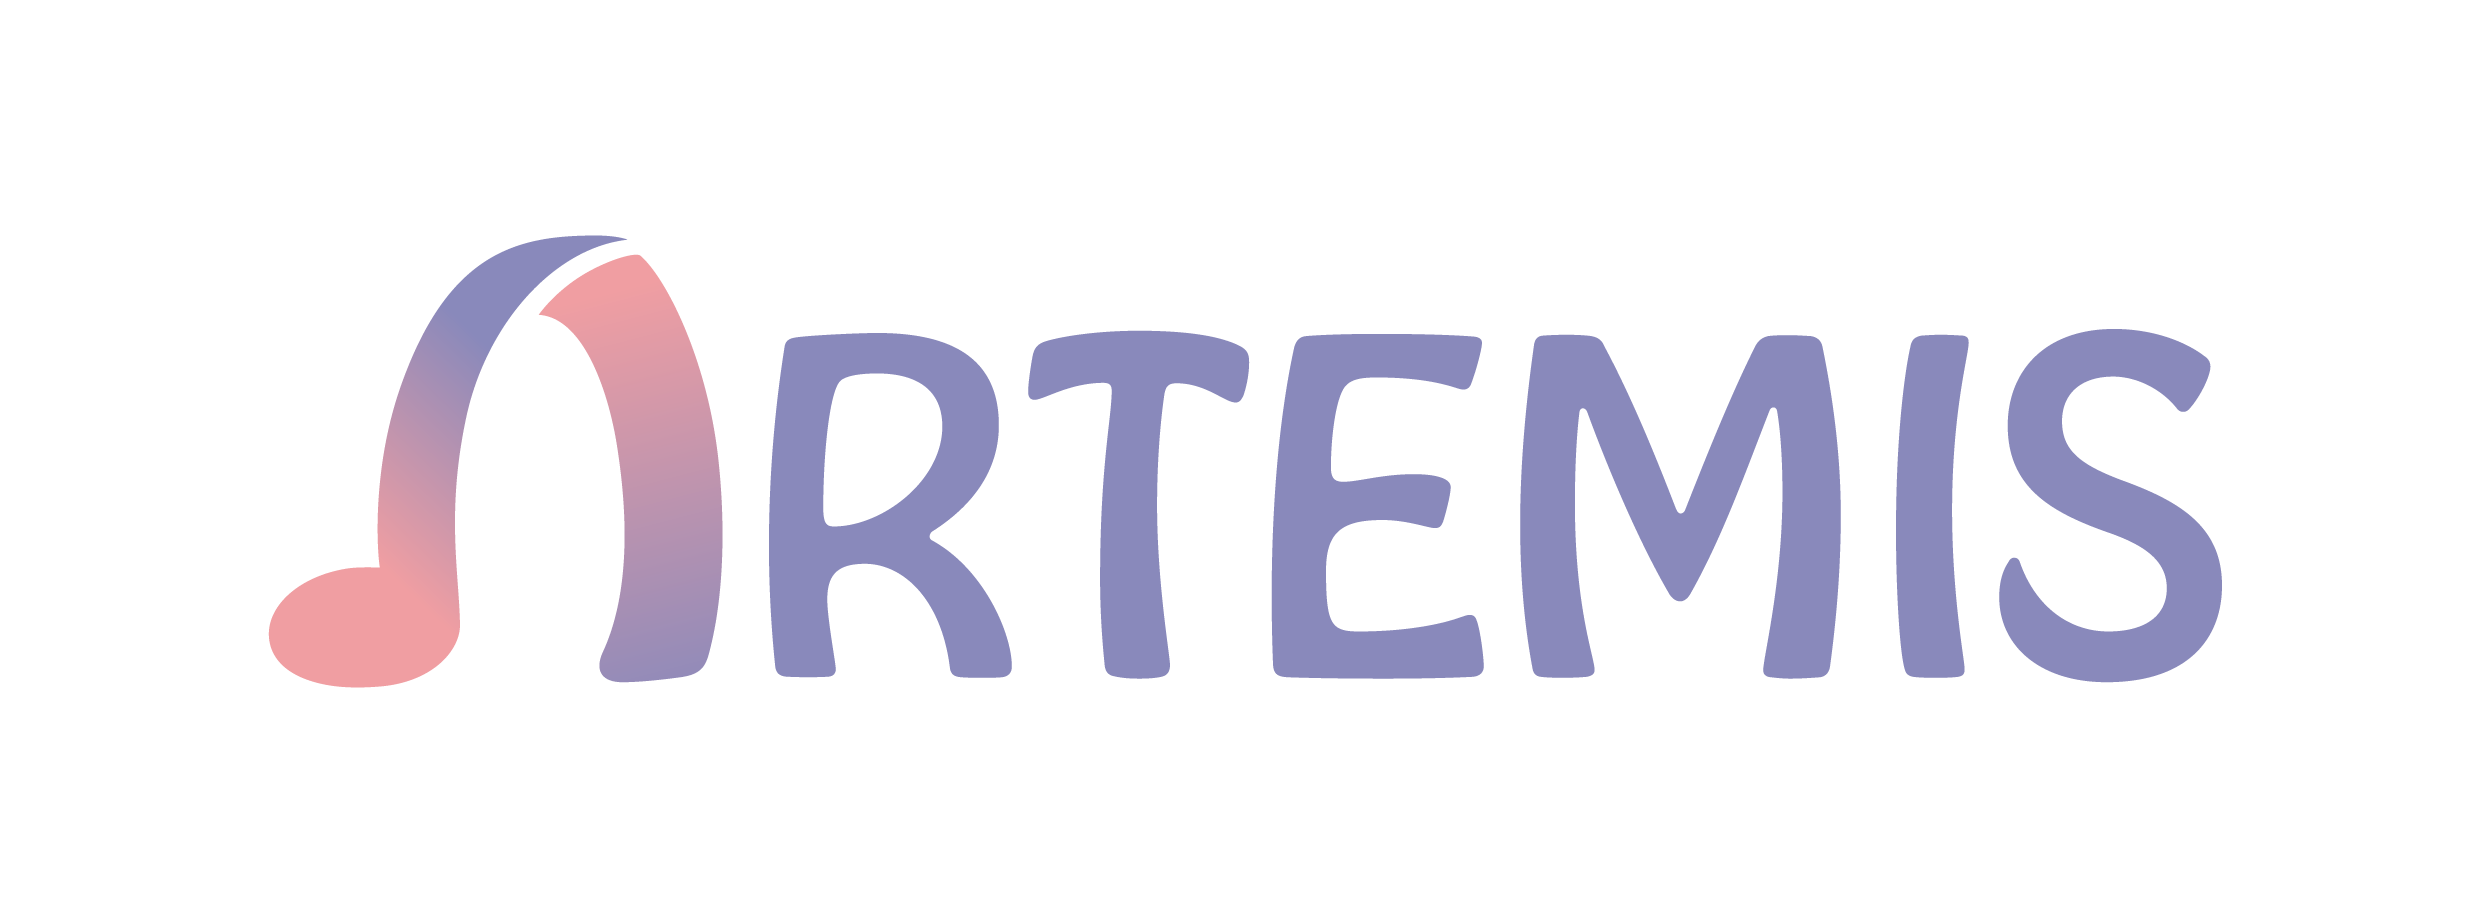
\includegraphics[width=0.9\linewidth]{Figuras/Introduccion/1_LogoArtemis}
	\caption{Logotipo del proyecto ARTEMIS.}
	\label{fig:logoArtemis}
\end{figure}

\section{Justificación y contexto}

El proyecto ARTEMIS se crea con el propósito de proporcionar soporte digital a las terapias psicológicas que tienen como objetivo utilizar la musicoterapia como medio para facilitar la transición entre estados emocionales. Su función radica en ser una herramienta complementaria que los terapeutas pueden implementar junto a las terapias más tradicionales, adaptándola a las necesidades de cada paciente. La aplicación, que conglomera las distintas experiencias, no debe ser utilizada solo por el paciente. Tiene un enfoque de doble usuario, donde ambas partes tienen su rol definido en la terapia. El paciente interactúa con la aplicación siguiendo las indicaciones del terapeuta, quién recogerá información relevante tanto antes como después de la interacción. De este modo, puede recibir feedback a tiempo real y redirigir las sesiones terapéuticas si fuera necesario. Además, el terapeuta tiene acceso a un registro que le permite observar la progresión del paciente. Esto le ayuda a identificar patrones y a priorizar los elementos que funcionan mejor en cada caso específico.

La investigación busca aportar una síntesis entre el diseño de productos interactivos y la musicoterapia, fundamentada por estudios previos sobre el uso de la música en el tratamiento de trastornos emocionales, en particular, la ansiedad. Esta emoción fue seleccionada para su estudio debido a su prevalencia en la sociedad y a su presencia a lo largo de la vida de una persona, teniendo un gran impacto, especialmente en la etapa de la niñez y adolescencia. Un estudio conducido por \citeauthor{MO:2012} (\citeyear{MO:2012}) indica que, de una muestra de aproximadamente 2500 niños y adolescentes entre 8 y 17 años (51\% de sexo femenino), de diversas nacionalidades (aunque predominantemente española) y diferentes situaciones socioeconómicas, el 26,41\% presentó puntuaciones altas en algún tipo de ansiedad. Aunque se hable de esta emoción como una única, \citeauthor{CAGD:2010} (\citeyear{CAGD:2010}) explica que se caracteriza por ser un conjunto de diferentes tipos que surgen como reacción a eventos o situaciones. Estos tipos están condicionados por las circunstancias que rodean al individuo y los recursos que tiene, conocidos como estrategias de afrontamiento. Entre las reacciones a la ansiedad se incluyen la incertidumbre, la impotencia y la activación fisiológica, fuertemente relacionadas con síntomas corporales de tensión y preocupación acerca del futuro. Los síntomas pueden intensificarse significativamente cuando se combina con la depresión, llegando incluso a la somatización. Como explica \citeauthor{CJI:2017} (\citeyear{CJI:2017}), la ansiedad puede hacer que la mente enferme al cuerpo. Aunque aún no podemos explicar el origen de las causas, el dolor y sufrimiento se manifiestan de forma real. 

La música y la salud están estrechamente relacionadas. La combinación adecuada de elementos musicales como tonos, ritmos y armonías puede impactar positivamente las condiciones físicas, fisiológicas y psicológicas de las personas. Aquí es donde entra la musicoterapia, un enlace entre el terapeuta y el paciente que busca cumplir un objetivo terapéutico específico a través de la interacción con medios musicales. En nuestro caso de estudio, el objetivo es reducir la ansiedad. \citeauthor{KTN:2011} (\citeyear{KTN:2011}) explica que los patrones de las ondas cerebrales cambian según el estado de ánimo del paciente que, combinados con ciertos tipos de música, pueden generar un equilibrio que conduce a la relajación. En los últimos años, se han empezado a implementar nuevas estrategias dentro de las sesiones de musicoterapia, incluyendo el uso de videojuegos como medio interactivo.

\section{Motivación}

La elección de la temática para este Trabajo de Fin de Grado se debe a la fusión de dos de mis mayores pasiones: los videojuegos y la música. Desde una edad temprana, ambos han jugado un papel crucial en mi vida, no solo como formas de entretenimiento, sino como medios de expresión y canales que me han servido para desarrollar la creatividad. La influencia personal de estas dos áreas se puede apreciar tanto desde la perspectiva del desarrollador o intérprete, como desde el punto de vista del jugador u oyente. El diseño y desarrollo de experiencias interactivas para la musicoterapia es el punto de convergencia de estas dos pasiones, donde se agrega el elemento psicológico, un tema de especial interés para mí. 

A través de la investigación y desarrollo de esta experiencia interactiva, pretendo potenciar mis conocimientos en los campos específicos a los que me gustaría dedicarme profesionalmente en la industria del videojuego. Este proyecto no solo me permitirá aplicar las habilidades técnicas y creativas que he ido desarrollando a lo largo de mi carrera educativa, sino que también me proporcionará una comprensión más profunda de cómo la música puede ser utilizada de manera terapéutica dentro de estos entornos interactivos. Además, me ayudará a comprender cómo, recopilar y analizar datos sobre la respuesta del usuario y los resultados terapéuticos, permite adaptar las sesiones terapéuticas al paciente a tiempo real, lo que fortalecerá mis habilidades de evaluación.

Mi gran curiosidad por la mente humana, que considero una pieza clave en la máquina perfecta que es el cuerpo humano, me impulsa a explorar cómo estas aplicaciones interactivas pueden influir en el cerebro y el comportamiento. Este proceso también me aportará información que alimente esta curiosidad en los campos psicológicos. Al investigar cómo las experiencias interactivas basadas en la música pueden influir psíquica y fisiológicamente, espero descubrir nuevas maneras en las que la tecnología puede ser utilizada para mejorar la salud mental y el bienestar general. Esta exploración que entrelaza disciplinas no solo enriquecerá mi formación académica y profesional, sino que también contribuirá a un campo de estudio en constante evolución, con el potencial de tener un impacto positivo y duradero en la vida de las personas.

\section{Planteamiento del problema}

La musicoterapia, tal como la conocemos hoy, se originó en la segunda mitad del siglo XIX. Sin embargo, las civilizaciones antiguas ya utilizaban la música como un medio divino para apaciguar a los dioses, vinculando la enfermedad con la maldad y la ofensa a estos (\citeauthor{JIPS:2001}, \citeyear{JIPS:2001}). Está claro que la musicoterapia ha sido una parte esencial de la vida humana durante milenios. A lo largo de la historia, variadas culturas han reconocido el poder curativo de la música, desde los rituales chamánicos de las tribus indígenas hasta las complejas composiciones de la Grecia clásica, donde filósofos como Pitágoras exploraron los efectos de los sonidos en el alma y el cuerpo.

Sin embargo, debido a la relativa reciente aparición de los medios digitales en comparación con la larga historia de la musicoterapia, el desarrollo de terapias interactivas digitales que utilizan la música como elemento central está en proceso de crecimiento. Esto implica que, a pesar del incremento de uso de este formato en diversas áreas científicas y el constante desarrollo de este tipo de experiencias, aún no ha logrado establecerse completamente en el área psicológica.

Actualmente, existen pocas investigaciones recientes sobre el uso de medios interactivos electrónicos en sesiones de musicoterapia, a pesar de su creciente presencia en otros sectores científicos, incluyendo otras áreas de la psicología. Esta brecha en la investigación representa una oportunidad significativa para explorar y desarrollar nuevas metodologías que integren eficientemente la tecnología digital con prácticas terapéuticas tradicionales. Las experiencias digitales interactivas tienen el potencial de ofrecer entornos controlados y adaptativos que pueden personalizarse para las necesidades individuales de cada uno de los pacientes, algo que puede ser más difícil de lograr con los métodos tradicionales.

El límite del diseño de videojuegos se encuentra en la imaginación del propio creador. Al combinar terapias tradicionales con medios digitales, se abre un rango más amplio de posibilidades terapéuticas. Esta combinación compensará las limitaciones físicas con las ventajas digitales, aprovechando lo mejor de ambos mundos. Es importante destacar que el formato digital no tiene como objetivo reemplazar las terapias tradicionales, sino funcionar como una herramienta complementaria que el terapeuta puede utilizar en sus sesiones, adaptándolas a las necesidades de cada paciente. Además, la interacción digital introduce nuevas formas de involucrar a los pacientes, manteniendo la interacción física del terapeuta con el paciente, permitiendo medir su progreso de manera objetiva, y lo que es más importante, en tiempo real.

\section{Objetivos del trabajo}

Teniendo en cuenta las motivaciones y problemas que se han planteado en los epígrafes anteriores, los objetivos que el trabajo pretende alcanzar son los siguientes:

\subsection{Objetivos generales}

\begin{itemize}
	
	\item Desarrollar una aplicación con enfoque de juego serio que incorpore elementos de musicoterapia y que pueda ser utilizado en sesiones terapéuticas y que tengan como objetivo mejorar el estado emocional con respecto a la ansiedad.
\end{itemize}

\subsection{Objetivos específicos}

\begin{itemize}
	\item Aportar una experiencia interactiva para complementar y mejorar las prácticas tradicionales.
	\item Estudio de patrones rítmicos, música, para permitir que el usuario cree/componga música.
	\item Investigar cómo las experiencias interactivas digitales pueden complementar y mejorar las prácticas tradicionales dentro del área psicológica de la musicoterapia.
\end{itemize}